\chapter{Интеграл} \index{Интеграл}
\section{Интегралын тодорхойлолт}
$\gamma :[\alpha,\beta]\rightarrow \mathbb{C}$ (Ийм буулгалтыг зам гэж нэрлэдэг) ба $f\in C(D)$ функц авч үзье. $\gamma ([\alpha, \beta])\subset D$ байг. $T$ нь $[\alpha, \beta]$ интервалийн хуваалт байг.
$$T=\{t_k:k\in\overline{0,n} \quad \text{ба} \quad \alpha =t_0<t_1<\ldots <t_n=\beta\}$$
$z_k=\gamma(t_k)$ ба $\textrm{\normalfont{diam} }T=\max\limits_{k\in \overline{1,n}} (t_k-t_{k-1})$ тэмдэглээнүүд оруулъя. Мөн $k\in\overline{1,n}$ бүрийн хувьд $\tau _k \in [t_{k-1}, t_k]$ сонгосноор $\zeta =\{ \zeta_k:\zeta_k=\gamma(\tau_k)\}$ олонлог байгуулъя (Үүнийг сонголт гэж нэрлэдэг).
\begin{eqnarray}
  S(f,\gamma ,T,\zeta)=\sum\limits_{k=1}^n f(\zeta_k)\cdot (z_k-z_{k-1})
\end{eqnarray}
хэмжигдэхүүнийг $f$ функцийн хувьд $\gamma$ замын $T$ хуваалт ба $\zeta$ сонголтоор зохиогдсон интеграл нийлбэр гэнэ.
\begin{dfn}
 \textbf{(Комплекс интеграл)}. Хэрэв $T$ ба $\zeta$ сонголтыг хэрхэн байгуулснаас үл хамаарч
 \begin{eqnarray}
   \exists \lim\limits_{\textrm{\normalfont{diam} }T\rightarrow 0}S(f,\gamma, T,\zeta)=I\in\mathbb{C}
 \end{eqnarray}
 бол I комплекс тоон утгыг $f$ функцээс $\gamma$ замаар авсан интеграл гэж нэрийдээд  $$I=\int\limits_\gamma f(z)dz$$ гэж тэмдэглэдэг.
\end{dfn}
\begin{thm}
 \textbf{(Интеграл орших зайлшгүй нөхцөл.)} $\gamma$ нь гөлгөр зам ба $f$ нь уг замын муруй дээр тасралтгүй бол
 \begin{eqnarray} \label{4.3}
   \exists \int\limits_{\gamma} f(z)dz=\int\limits_\alpha^\beta f(\gamma(t))\cdot \gamma '(t)dt 
 \end{eqnarray}
 байна. (\ref{4.3}) томьёог интеграл бодох параметрчилэлийн томьёо гэдэг.
\end{thm}
\begin{prf}
$\gamma (t)=a(t)+ib(t)$ ба $\gamma$ гөлгөр гэдгээс $a(t)$, $b(t)\in C^{(1)}[\alpha,\beta]$ болж Лагранжийн томьёог ашиглах боломжтой.
$$
\begin{cases}
a(t_k)-a(t_{k-1})=a'(\xi_k)(t_k-t_{k-1}) \\
b(t_k)-b(t_{k-1})=b'(\xi_k')(t_k-t_{k-1}), \quad (\xi_k,\xi_k'\in[t_{k-1},t_k]) 
\end{cases}
$$ 

болно.

$a'$, $b'\in C[\alpha,\beta]$ учир Канторын теоремоор жигд тасралтгүй байх ёстой. $\forall \varepsilon >0 \exists \delta >0 \quad \forall t_1,$ $t_2\in [\alpha, \beta]$ хувьд $|t_1-t_2|<\delta$ бол $|a'(t_1)-a'(t_2)|<\varepsilon$; $|b'(t_1)-b'(t_2)|<\varepsilon$ болно. Хуваалтын диаметрийг $\delta$-с багаар авбал 
\begin{align*}
    &\left|\sum\limits_{k=1}^n f(\zeta_k)(\gamma(t_k)-\gamma(t_{k-1}))-\sum\limits_{k=1}^nf(\zeta_k)\gamma'(\tau_k)(t_k-t_{k-1})\right|=\\
    &=\left| \sum\limits_{k=1}^n f(\zeta_k)(a'(\xi_k)-a'(\tau_{k}))+i\sum\limits_{k=1}^nf(\tau_k)(b'(\xi'_k)-b(\tau_{k}))\right|\leq \\
    &\leq 2\varepsilon \max\limits_{z\in \gamma [\alpha,\beta]}|f(z)|\cdot (\beta-\alpha)
\end{align*}
болно.

$\varepsilon$-г дураар сонгож болох учир
$$\left|\int\limits_\gamma f(z)dz-\int\limits_\alpha^\beta f(\gamma(t))\gamma '(t)dt\right|=0$$
болж теорем батлагдав. 
\end{prf} 
\begin{cor}
$$\int\limits_\gamma f(z)dz=\int\limits_\gamma udx-vdy+i\int\limits_\gamma vdx+udy.$$
\end{cor}
\begin{cor}
$\gamma$ нь хэсэгчилсэн гөлгөр зам үед дээрх теорем хүчинтэй.
\end{cor}
\begin{exm} \label{Example z^n int}
$\gamma$ нь $a\in\mathbb{C}$ төвтэй $R$ радиустай тойргийг цагийн зүүний эсрэг 1 эргэсэн $\gamma(t)=a+R\cdot e^{it}(t\in[0;2\pi])$ зам байг.
\begin{align*}
    \int\limits_\gamma (z-a)^n dz&=\int\limits_{0}^{2\pi} ((a+Re^{it})-a)^n\cdot(a+Re^{it})'_tdt \\
    &=R^{n+1}\cdot i\int\limits_0^{2\pi} [\cos (n+1)t+i\sin (n+1)t]dt \\
    &=
    \begin{cases}
    0, \quad n\neq -1, \\
    2\pi i, \quad n=-1
    \end{cases}
\end{align*}
\end{exm}
\begin{exm}
$\gamma(t)=t+it^2(t\in [0;1])$ параболын нумаар 
\begin{align*}
    \int\limits_\gamma \re (z^2)dz&=\int\limits_0^1 \re (t+it)^2\cdot (t+it^2)_t'dt \\
    &=\int\limits_0^1 (t^2-t^4)(1+2itdt) \\
    &=\dfrac{2}{15}+\dfrac{1}{6}\cdot i
\end{align*}
\end{exm}
\begin{exm}
$\gamma$ нь $z_0$ цэгээс $z_1$ хүрсэн хэрчим зам \\ $\gamma(t)=z_0+(z-1-z_0)t$ \quad $(t\in[0,1])$ байг.
\begin{align*}
    \int\limits_{\gamma^+}(az+b)dz&= \int\limits_0^1 [a(z_0+(z_1-z_0)t)+b]\cdot (z_0+(z_1-z_0)t)'_tdt \\
    &=a\dfrac{z_1^2-z_0^2}{2}+b(z_1-z_0).
\end{align*}
\end{exm}
\begin{exm} \label{Жишээ 4}
Гурвалжны хилээр тойрсон зам контур $\partial \Delta^+$ (битүү замыг контур гэж нэрлэх нь байдаг) бол $$\bint\limits_{\partial\Delta^+} (az+b)dz=0$$ байхыг жишээ 4.3-аас гаргана уу.
\end{exm}
\section{Комплекс интегралын чанарууд}
Энд $\gamma$ нь хэсэгчилсэн гөлгөр зам ба $f$, $g\in C(\gamma [\alpha, \beta])$ (замын муруй дээр тасралтгүй) функцүүд байг.
\begin{sen}
(Шугаман чанар) $\forall a,b\in\mathbb{C}$ хувьд
$$\int\limits_{\gamma} [af(z)+bg(z)]dz=a\int\limits_\gamma f(z)dz+b\int\limits _\gamma g(z)dz$$
байна.
\end{sen}
\begin{sen}
(Аддитив чанар) $\gamma =\gamma_1 \wedge \gamma_2$ бол 
$$\int\limits_{\gamma} f(z)dz=\int\limits_{\gamma_1} f(z)dz+\int\limits _{\gamma_2} f(z)dz$$
байна.
\end{sen}
\begin{sen} \label{Чанар 3}
$\gamma^{-}$ эсрэг замын хувьд
$$\int\limits_{\gamma^-}f(z)dz =-\int\limits_\gamma f(z)dz$$
\end{sen}
\begin{hnt}
Битүү замын (контур) хувьд зүүн гарын дүрмээр ориентацлаж чиглэл тогтоовол $\gamma^+$ гэж тэмдэглэдэг.
\end{hnt}
\begin{center}
 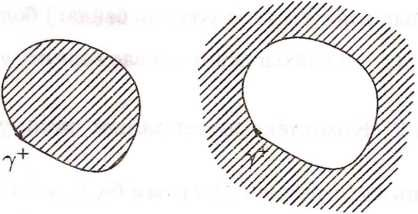
\includegraphics[width=6cm]{Zurag/8.jpg}  
 \captionof{figure}{}
        \label{ref hiih ner}
\end{center}
\begin{prf}
Комплекс интеграл нь муруй шугаман 2-р төрлийн интегралаар илэрхийлэгддэг нь теорем 1-ийн мөрдлөгөө болсон. Мөн дээрх чанарууд түүнийх нь хувьд биелдгийг Математик анализын хичээл дээр үзсэнээ санавал чанарууд батлагдаж байна.
\end{prf}
\begin{sen}
(Интегралыг үнэлэх).
$$\left|\int\limits_\gamma f(z)dz\right|\leq \int\limits_\gamma |f|dl\leq |\gamma|\cdot \max\limits_{z\in\gamma [\alpha,\beta]}|f|.$$
\end{sen}
\begin{prf}
$|dz|=\sqrt{(dx)^2+(dy)^2}=dl$ (Уртын дифференциал) байна.

Иймд гурвалжны тэнцэл биш ашиглавал
$$\left|\int\limits_\gamma f(z)dz\right|\leq \int\limits_\gamma \left|f(z)dz\right|=\int\limits_l |f(z)|dl$$ болж эхний тэнцэл биш
батлагдав.

Эерэг функцээс уртын дифференциалаар авч байгаа учир
$$\int\limits_\gamma \left(\max\limits_{z\in \gamma[\alpha, \beta]}|f|-|f(z)|\right)dl\leq 0\Rightarrow$$
$$\int\limits_\gamma|f(z)|dl\leq \int\limits_\gamma \max_{z\in \gamma [\alpha,\beta]}|f|dl=\max\limits_{z\in \gamma[\alpha,\beta]}|f|\int\limits_\gamma dl=\left(\max\limits_{z\in\gamma [\alpha,\beta]}|f|\right) \cdot |\gamma|$$
болж дараагийн тэнцэл биш батлагдав.
\hfill \end{prf}
\section{Кошийн интеграл теорем} \index{Кошийн интеграл теорем}
\begin{thm}
\textbf{ (Гурвалжин контурын Кошийн теорем).} $f\in H(D)$ ба дотоод муж нь хилийн хэрчмүүдтэйгээ $D$ мужид агуулагдсан гурвалжин $\Delta$ авъя $(\overline{\Delta}\subset D)$. Тэгвэл 
$$\int\limits_{\partial \Delta^+}f(z)dz=0$$
байна. 
\end{thm}
\begin{prf}
Эсрэгээс нь $\exists \Delta_0:\overline{\Delta_0}\subset D$ боловч \\ $\left|\bint\limits_{\partial \Delta_0^+}f(z)dz\right|=M>0$ гэж үзье.
\begin{center}
 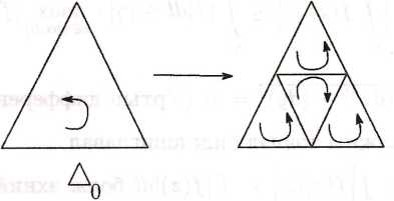
\includegraphics[width=6cm]{Zurag/9.jpg}  
 \captionof{figure}{}
        \label{ref hiih ner}
\end{center}
Гурвалжныг зурагт үзүүлсэн аргаар дундаж шугамуудаар нь хуваавал Чанар 4.3 ёсоор $\bint\limits_{\partial \Delta_0^+} f(z)dz$ нь дөрвөн интегралын нийлбэр болж сална. Иймд эдгээрээс модуль нь $\dfrac{M}{4}$ багагүй байх дор хаяж нэг гурвалжин сонгогдож чадна. Үүнийг нь $\Delta_1$ гэе. 
$$\left|\int\limits_{\partial \Delta_1^+} f(z)dz\right|\geq \frac{M}{4}$$
Энэ алхмыг үргэлжлүүлэн $n$ удаа хийсэн гэвэл $\exists \Delta_n:\Delta_n$ нь $\Delta_0$ гурвалжингаас $2^n$ дахин төсөөтэйгөөр багассан ба 
\begin{equation}
    \tag{$*$} \label{*}
    \left|\int\limits_{\partial \Delta_n^+} f(z)dz\right|\geq \frac{M}{4^n}
\end{equation}
байна.

Багталцсан бөмбөрцгүүдийн зарчим ёсоор 
$$\exists z_0\in D:z_0=\bigcap\limits_{n=1}^\infty \overline{\Delta_n} $$
байна.
$f\in H(d)$ нөхцөл ёсоор 
$$\forall \varepsilon >0: \exists \delta>0 \forall z\in U=\{|z-_0|<\delta\}\cap D$$ хувьд
$$
\begin{cases}
 f(z)=f(z_0)+f'(z_0)(z-z_0)+\alpha (z)(z-z_0) \\
 |\alpha (z)|<\varepsilon
\end{cases}
$$ байна. 
$\Delta_0\subset U$  гэж үзэхэд явцуурахгүй нь ойлгомжтой. Иймд
$$\int\limits_{\partial \Delta_n}f(z)dz=\int\limits_{\partial \Delta_n} [f(z_0)+f'(z_0)(z-z_0)]dz+\int\limits_{\partial \Delta_n}\alpha (z)(z-z_0)dz$$
ба жишээ 4.4 ёсоор эхний нэмэгдэхүүн тэг болно. Харин дараагийн нэмэгдэхүүнийг үнэлбэл
\begin{equation}
\tag{$**$} \label{**}
    \begin{split}
    \left| \int\limits_{\partial \Delta_n}\alpha(z)(z-z_0)dz\right|&\leq \max |\alpha(z)|\cdot \max_{z\in \partial \Delta_n}|z-z_0|\cdot P_{{\Delta_n}}< \\
    &<\varepsilon \cdot P_{\Delta_n}\cdot P_{\Delta_n}=\varepsilon\cdot \frac{P^2_{\Delta_0}}{4^n}
\end{split}
\end{equation}
байна. (Энд $P_{\Delta_n}$ нь $\Delta_n$ гурвалжны периметрийг авав). ($*$) (\ref{**}) тэнцэл бишүүдээс
$$\frac{M}{4^n}<\varepsilon \frac{P^2_{\Delta_0}}{4^n}\Rightarrow \frac{M}{P^2_{\Delta_0}}<\varepsilon$$
болж $\varepsilon$ дураараа сонгож болно гэдэгтэй харшилдав. Иймээс Кошийн теорем гурвалжин контурын хувьд батлагдаж байна.
\hfill \end{prf}
\begin{thm} \label{Теорем 3}
\textbf{(Тахир шугаман контурын Кошийн теорем).} $f\in H(D)$, $\gamma$ нь битүү жорданы тахир шугам (дотоод мужийн хамт $D$ мужид оршдог) байг. Тэгвэл $\bint\limits_{\gamma^+}f(z)dz=0$ байна.
\end{thm}
\begin{prf}
Аливаа тахир шугамыг дотоод диагональ татсаар төгсгөлөг тооны гурвалжнуудад хувааж (триангуляци хийж) болдгийг дасгал болгон батална уу. Тэгвэл интегралын аддитив чанар ёсоор $\bint\limits_{\gamma^+} f(z)dz$ нь гурвалжны хилээр авсан интегралуудын нийлбэрт задарна. Одоо Теорем 4.2 ашиглавал энэ теорем батлагдана. 
\hfill  \end{prf}
\begin{thm} \label{Теорем 4}
\textbf{(Гөлгөр контурын Кошийн теорем).} \\ $f\in H(D)$, $\gamma$ нь битүү жорданы гөлгөр зам (дотоод мужтайгаа хамт $D$ мужид оршдог) байг. Тэгвэл $\bint\limits_{\gamma^+}f(z)dz=0$ байна.
\end{thm}
\begin{prf}
Интеграл нийлбэр зохиох дурын $T$ хуваалт нь битүү тахир шугам өгнө. Энд Теорем 4.3-г ашиглах хэрэгтэй. 
\hfill  \end{prf}
\begin{dfn}
 $D$ муж өгөгдсөн.$\gamma_1:[0,1]\rightarrow D$,\\ $\gamma_2:[0,1]\rightarrow D$ замуудын хувьд $\gamma_1(0)=\gamma_2(0)$, $\gamma_1(1)=\gamma_2(1)$  ба 
 $$\exists \gamma (t,s)\in C ([0,1]^2\rightarrow D):\gamma_1(t)=\gamma (t,0); \quad \gamma_2(t)=\gamma(t,1)$$
 бол  $\gamma_1$, $\gamma_2$ замуудыг $D$ мужид нэг эхлэл төгсгөлтэй гомотоп замууд гэж нэрлээд $\gamma_1 \undertilde{D} \gamma_2$ тэмдэглэдэг.
\end{dfn}
\begin{dfn}
 $D$ муж өгөгдсөн. $\gamma_1:[0,1]\rightarrow D$,\\ $\gamma_2:[0,1]\rightarrow D$ замуудын хувьд $\gamma_1(0)=\gamma_1(1)$ ба $\gamma_2(0)=\gamma_2(1)$  ба 
 $$\exists \gamma (t,s)\in C ([0,1]^2\rightarrow D):\gamma_1(t)=\gamma (t,0); \quad \gamma_2(t)=\gamma(t,1)$$
 бол  эдгээр замуудыг $D$ мужид битүү замын гомотоп гэж нэрлээд $\gamma_1\undertilde{D} \gamma_2$ тэмдэглэдэг.
\end{dfn}
\begin{center}
 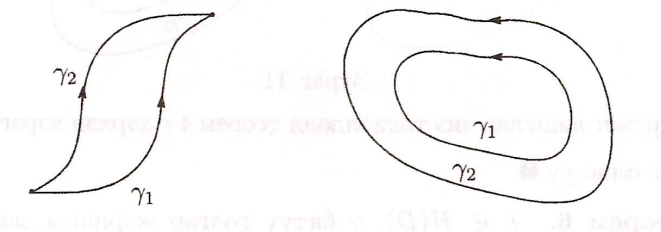
\includegraphics[width=8cm]{Zurag/10.PNG}  
 \captionof{figure}{}
        \label{ref hiih ner}
\end{center}
\begin{cor} 
Теорем 4.4-г дараах байдлаар өөрчлөн томьёолж болно. $f\in H(D)$ нь битүү гөлгөр Жорданы зам ба $\gamma \undertilde{D} 0$ бол
$\bint\limits _\gamma f(z)dz=0$ байна.
\end{cor}
\begin{thm} \label{Теорем 5}
\textbf{(Кошийн теоремын гомотоп хэлбэр).} \\ $f\in H(D)$, $\gamma_1 \undertilde {D} \gamma_2$ гөлгөр замууд байг. Тэгвэл $$\int\limits_{\gamma_1} f(z)dz =\int\limits_{\gamma_2} f(z)dz$$ байна.
\end{thm}
\begin{prf}
Эхлээд $\gamma_1\undertilde{D}\gamma_2$ эхлэл төгсгөл давхацсан гомотоп байг. Теорем 4.4 ёсоор $\bint\limits_{\gamma_1\wedge \gamma_2^{-}} f(z)dz=0$. Улмаар 
$$\int\limits_{\gamma_1}f(z)dz-\int\limits _{\gamma_2} f(z)dz=0$$
болж теорем батлагдана.

Одоо $\gamma_1\undertilde{D}\gamma_2$ битүү замын гомотоп байг.
\begin{center}
 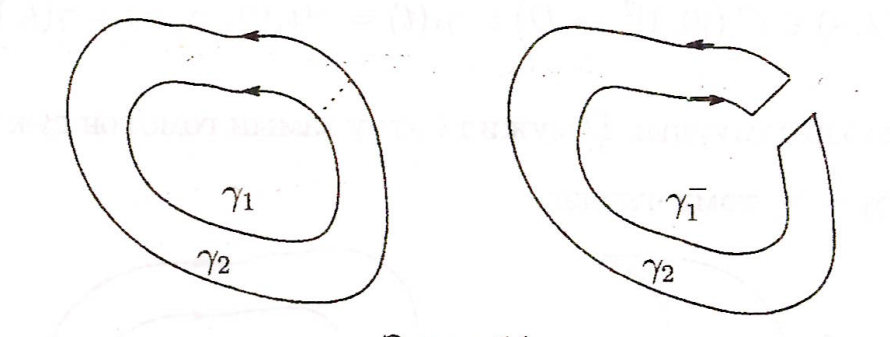
\includegraphics[width=8cm]{Zurag/11.PNG}  
 \captionof{figure}{}
        \label{ref hiih ner}
\end{center}
Зургийг ажиглан энэ тохиолдолд Теорем 4.4-г хэрхэн хэрэглэхийг олно уу.
\hfill  \end{prf}
\begin{thm}\label{removeablediscontinousfunctionint}
$f\in H(D)$, $\gamma$ битүү гөлгөр жорданы зам ба түүний дотоод мужийг $int \gamma$ гэж тэмдэглэе. $z_0\in int \gamma$ хувьд $z_0\notin D$ ба $(\overline{in t \gamma}\setminus \{z_0\})\subset D$ байг. Харин $f$ функцийн хувьд $z_0$ засагдах тасралтын цэг (өөрөөр хэлбэл $\exists \lim\limits_{z\rightarrow z_0}f(z)=a\in \mathbb{C})$ байг. Тэгвэл $\bint\limits_\gamma f(z)dz=0$ байна.
\end{thm}
\begin{prf}
$C_\varepsilon (z_0)$ нь $z_0$ төвтэй $\varepsilon$ радиустай тойрог байг. $\varepsilon$ хангалттай бага үед $\gamma \undertilde{D} C_{\varepsilon} (z_0)$ тул Теорем 4.5 ёсоор $$\int\limits_{\gamma}f(z)dz=\int\limits_{C_\varepsilon (z_0)} f(z)dz$$
ба $$\left|\int\limits_{C_\varepsilon(z_0)} f(z)dz\right|\leq 2\pi \cdot \varepsilon \cdot \max_{z\in C_{\varepsilon} (z_0)}|f(z)| =2\pi \cdot \varepsilon (|a|+\circ (1))$$
болно. $\varepsilon$-г хэчнээн ч багаар сонгож болох тул байна. 
$$\int\limits_{\gamma} f(z)dz=0$$ байна. 
\hfill  \end{prf}
\begin{thm}
\textbf{(Олон холбоост мужийн Кошийн теорем).} \index{Олон холбоост муж дахь Кошийн интеграл теорем} $D$ нь $n$ холбоост зааглагдсан муж ба $f\in H(D)\cap C(\overline{D})$ байг. Тэгвэл $$\bint\limits_{\partial D^+} f(z)dz=0$$ байна.
\end{thm}
\begin{prf}
Теорем 4.4-рүү хэрхэн шилжүүлж байгааг зургаас харна уу.
\begin{center}
 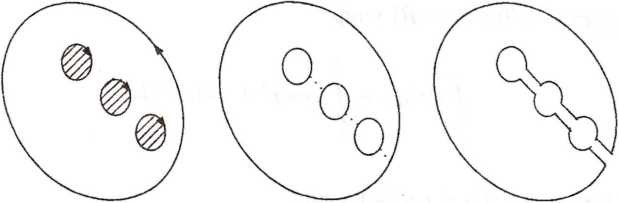
\includegraphics[width=8cm]{Zurag/12.jpg}  
 \captionof{figure}{}
        \label{ref hiih ner}
\end{center}
\hfill  \end{prf}
\begin{hnt}
Кошийн интеграл теоремууд нь гармоник функцийн хувьд хүчинтэй байдаг. 
\end{hnt}
\begin{exm}
$I=\bint\limits_0^{+\infty}\cos x^2dx$; $J=\bint\limits_0^{+\infty}\sin x^2dx$ интегралуудын утгыг тооцоол.
\end{exm}
\begin{sol}

Зурагт үзүүлсэн секторын хил контурыг $\gamma^+$ гэе.
$$\gamma^+=\gamma^+_1\vee \gamma_2^+\vee \gamma_3^+$$ 
$\gamma^+$ нь 2 хэрчим, 1 тойргийн нумаас тогтоно.
\begin{center}
    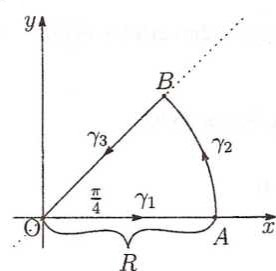
\includegraphics [width=6cm]{Zurag/13.jpg}
 \captionof{figure}{}
        \label{ref hiih ner}
\end{center}
Кошийн теорем ёсоор
\begin{equation}
\tag{$*$} \label{7*}
  0=\int\limits_{\gamma^+} e^{iz^2}dz=\int\limits_{\gamma_1^+} e^{iz^2}dz+\int\limits_{\gamma_2^+} e^{iz^2}dz+\int\limits_{\gamma_3^+} e^{iz^2}dz
\end{equation}
 $\gamma^+_1 (x)=x(0\leq x\leq R)$ учир 
$$\int\limits_{\gamma_1^+} e^{iz^2}dz=\int\limits_{0}^R(\cos x^2+i\sin x^2)dx$$
$\gamma^+_2 (t)=Re ^{it}(0\leq t\leq \dfrac{\pi}{4})$ учир 
$$\int\limits_{\gamma_2^+} e^{iz^2}dz=\int\limits_{0}^{\frac{\pi}{4}}e^{-R^2\sin 2t+iR^2\cos 2t}\cdot Re^{it}\cdot idt$$
ба 
$$\left|\int\limits_{\gamma_2^+}e^{iz^2}dz\right|  \leq R\int\limits_{0}^\frac{\pi}{4} r^{-R^2\sin 2t}dt\leq R\int\limits_0^{\frac{\pi}{4}}e^{-R^2\frac{2}{\pi}2t}dt=\dfrac{\pi}{4}\cdot \frac{1-e^{-R^2}}{R}$$
$\gamma_3^+(t)=t\left(\dfrac{1}{\sqrt{2}}+i\dfrac{1}{\sqrt{2}}\right) \quad (R\geq t\geq 0)$ учир 
\begin{align*}
    \int\limits_{\gamma_3^+}e^{iz^2}dz&=\int\limits_R^0 e^{-t^2}\cdot \left(\frac{1}{\sqrt{2}}+i\frac{1}{\sqrt{2}}\right) dt \\
    &=- \left(\frac{1}{\sqrt{2}}+i\frac{1}{\sqrt{2}}\right)\int\limits_0^Re^{-t^2}dt.
\end{align*}
 Одоо (\ref{7*}) тэнцэтгэлд $R\rightarrow +\infty$ шилжвэл
 $$0=(I+iJ)+0+\left(-\frac{1}{\sqrt{2}}-i\frac{1}{\sqrt{2}}\right) \int\limits_0^{+\infty} e^{-t^2} dt.$$
 Иймд
 $$J=I=\frac{1}{\sqrt{2}}\int\limits_0^{+\infty} e^{-t^2} dt=\frac{\pi}{2\sqrt{2}}.$$

\end{sol}
\begin{center}
    \textbf{Дасгал}
\end{center}
$f(z)=\dfrac{e^{iz}}{z}$ ба зурагд үзүүлсэн $\gamma^+$ контурыг ашиглан $\bint\limits_0^{+\infty} \dfrac{\sin x}{x}dx$	 тооцоол.
\begin{center}
    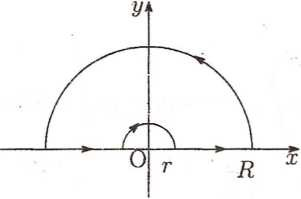
\includegraphics[width=6cm]{Zurag/14.jpg}
     \captionof{figure}{}
\end{center}
\section{Эх функц. Ньютон-Лейбницийн томьёо} \index{Ньютон-Лейбницийн томьёо}
\begin{thm}
$D$ гүдгэр муж ба $z_0\in D$ байг. $f\in H(D)$ үед $F(z)=\bint\limits_{z_0}^zf(z)dz$ томьёогоор функц тодорхойлогдох ба 
$F'(z)=f(z)$ байна. (Өөрөөр хэлбэл голоморф функц гүдгэр муж дээр эх функцтэй байна).
\end{thm}
\begin{prf}
Гүдгэр муж нэг холбоост байна. Иймд $z_0$ цэгээс гарч $z$ цэг дээр төгсгөлтэй бүх замууд гомотоп байна. Ийнхүү $\bint\limits_{z_0}^z f(z)dz$ ганц утгатай, функц тодорхойлж өгнө. Энэ замуудаас $[z_0,z]$ хэрчим дагуу шугаман зам авахад хангалттай (Энд гүдгэр ашиглагдана).
\begin{center}
    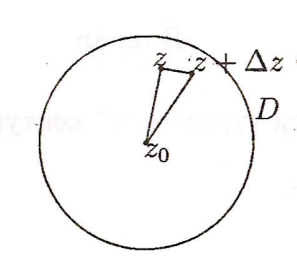
\includegraphics[width=4cm]{Zurag/15.jpg}
     \captionof{figure}{}
\end{center}
\begin{align*}
    \frac{f(z+\Delta z)-F(z)}{\Delta z}&=\frac{\int\limits_z^{z+\Delta z}f(z)dz}{\Delta z} \\
    &=\frac{\int\limits_0^1 f(z+\Delta z\cdot t)\Delta z dt}{\Delta z}=\int\limits_0^1 f(z+\Delta zt) dt;
\end{align*}
\begin{align*}
    \lim\limits_{\Delta z\rightarrow 0}\frac{F(z+\Delta z)-F(z)}{\Delta z}&=\int\limits_0^1 \left(\lim\limits_{\Delta z\rightarrow 0}f(z+\Delta z\cdot t)\right) dt \\
    &=\int\limits_0^1 f(z)dt= f(z)
\end{align*}
болж батлагдав. 
\hfill  \end{prf}
\begin{cor}
$D$ нэг холбоост муж $f\in H(D)$ бол $f$ нь $D$ муж дээр эх функцтэй байна.
\end{cor}
\begin{hnt}
Голоморф биш функцүүд муж дээр эх функцтэй байж чаддаггүй. $(w=|z| \quad w= \re z;\quad w=x+iy^3$ гэх мэт)
\end{hnt}
\begin{hnt}
$f\in H(D)$ боловч $D$ нэг холбоост бус үед эх функц олддог $\left( D=\mathbb{C}\setminus \{0\}, \quad f(z)=\dfrac{\sin z}{z}\right)$ ба эс оршдог \\ $\left(D=\mathbb{C}\setminus \{0\}, \quad f(z)=\dfrac{\cos z}{z}\right)$ жишээнүүд байдгийг анхаарах хэрэгтэй.
\end{hnt}
\begin{thm}
$\gamma:[\alpha, \beta]\rightarrow \mathbb{C}$ гөлгөр зам ба $f$ функц $\gamma$ замын дагуу $\Phi(z)$ эх функцтэй байг. Тэгвэл
\begin{eqnarray}
  \int\limits_\gamma fdz=\Phi (\gamma (\beta))-\Phi (\gamma (\alpha))
\end{eqnarray} байна.
\end{thm}
\begin{prf}
$$\int\limits_\gamma f(z)dz=\int\limits_\alpha^\beta f(\gamma (t))\gamma'(t)dt =\Phi (\gamma(t))\Big|_{\alpha}^\beta$$
\hfill  \end{prf} болно.
\section{Кошийн интеграл томьёо} \index{Кошийн интеграл томьёо}
\begin{thm}
\textbf{(Кошийн интеграл томьёо).} \\ $f\in H(D)$ ба $z_0\in D$ байг. 
$$V_{z_0} (r)=\{z:|z-z_0|<r\} \quad \text{ба} \quad \gamma^+\undertilde{D} \partial V_{z_0}^+ (r)$$ байг. Өөрөөр хэлбэл   $\gamma^+ \text{ ба } \partial V_{z_0}^+ (r)$ гомотопи замууд байг. Тэгвэл $$ \bint\limits_{\gamma^+}\dfrac{f(z)}{z-z_0}dz=2\pi i f(z_0).$$
\end{thm}
\begin{prf}
$$\frac{f(z)}{z-z_0}=\frac{f(z)-f(z_0)}{z-z_0}+\frac{f(z_0)}{z-z_0}$$ учир
$$\int\limits_{\gamma^+}\frac{f(z)}{z-z_0}dz=\int\limits_{\gamma^+}\frac{f(z)-f(z_0)}{z-z_0}dz+\int\limits_{\gamma+}\frac{f(z_0)}{z-z_0}dz$$ болно.

$f(z)$ функц $z_0$ цэг дээр голоморф учир $\varphi(z)=\dfrac{f(z)-f(z_0)}{z-z_0}$ функц нь $z_0$ цэг дээр засагдах тасралтттай. Иймд Теорем \ref{removeablediscontinousfunctionint} ёсоор $$\int\limits_{\gamma^+}\frac{f(z)-f(z_0)}{z-z_0}dz=0$$ болно.

Хэрэв Жишээ \ref{Example z^n int}-ийг $n=-1$ үед хэрэглэвэл 
$$\int\limits_{\gamma+}\frac{f(z_0)}{z-z_0}dz=\int\limits_{\partial V^+_{z_0}(r)}\frac{f(z_0)}{z-z_0}dz=f(z_0)\cdot\int\limits_{\partial V^+_{z_0}(r)}\frac{1}{z-z_0}dz=2\pi i f(z_0)$$ болно. Иймд 
$$\int\limits_{\gamma^+}\frac{f(z)}{z-z_0}dz =2\pi i f(z_0)$$ болж батлагдав.
\hfill  \end{prf}
\begin{cor}
\textbf{(Дунджийн теорем).} $f\in H(D)$ ба $z_0\in D$ байг. Тэгвэл $f(z_0)$ утга нь $z_0$ төвтэй хангалттай жижиг тойргийн цэгүүд дээрх функцийн утгуудын дундаж байна. Өөрөөр хэлбэл: $$f(z_0)=\frac{1}{2\pi}\int\limits_0^{2\pi}f(z_0+\varepsilon \cdot  e^{it} dt)$$ (Энд $\overline{V_{z_0}}\subset D$ байх ёстой).
\end{cor}
\begin{prf}
$\partial V^+_{z_0}(\varepsilon)$ хувьд $f(z_0)=\dfrac{1}{2\pi i}\int\limits_{\partial V^+_{z_0}(\varepsilon)}\dfrac{f(z)}{z-z_0}dz$ гэж Кошийн интеграл томьёо бичигдэнэ. Одоо уг тойргийг \\ $z=z_0+\varepsilon e^{it}\quad (0\leq t\leq 2\pi)$ гэж параметрчилбэл
\begin{align*}
    f(z_0)&=\frac{1}{2\pi i}\int\limits_{\partial V^+_z (\varepsilon)}\frac{f(z)}{z-z_0}dz=\frac{1}{2\pi i}\int\limits_0^{2\pi}\frac{f(z_0+\varepsilon e^{it})}{\varepsilon e^{it}}\cdot (\varepsilon e^{it})'_{t}dt\\
    &=\dfrac{1}{2\pi}\int\limits_{0}^{2\pi} f(z_0+\varepsilon e^{it})dt
\end{align*}
болж батлагдав. 
\hfill  \end{prf}
\begin{exm}
$\gamma$ нь $3i$ төвтэй $R\neq 6$ радиустай тойрог байг. $I(R)=\bint\limits_{\gamma^+}\dfrac{dz}{z^2+9}$ тооцоол.
\end{exm}
\begin{sol}
$\gamma_1=\partial V^+_{3i} (1)$ ба $\gamma_2=\partial V^+_{-3i} (1)$ байг. 
    \begin{enumerate}
    \item [a)] $0<R<6$ үед $\gamma^+\sim \gamma_1^+$ учир 
    \begin{align*}
        \int\limits_\gamma \frac{dz}{z^2+9}&=\int\limits_{\gamma_1^+}\frac{\left(\frac{1}{z+3i}\right)dz}{z-3i}\\
        &=2\pi i\cdot \frac{1}{3i+3i}=\frac{\pi}{3}
    \end{align*}
 гарна.
    \end{enumerate}
    \begin{center}
        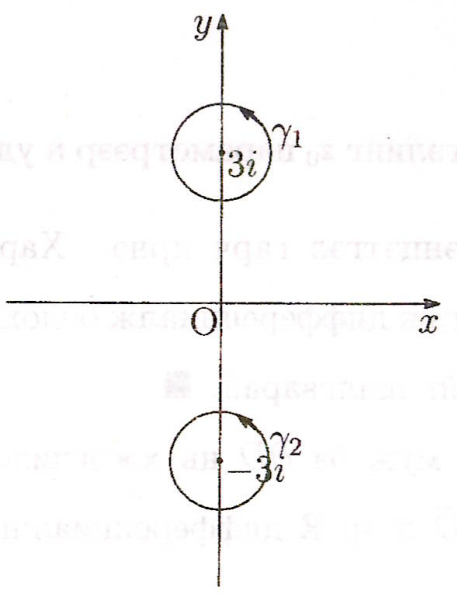
\includegraphics[width=5cm]{Zurag/16.PNG}
 \captionof{figure}{}
        \label{ref hiih ner}
    \end{center}
\begin{enumerate}
    \item [б)] $R>6$ үед $\gamma^+\sim \gamma_1^+\wedge \gamma_2^+$ тул 
    $$\int\limits_{\gamma^+}\frac{dz}{z^2+9}=\int\limits_{\gamma_1^+}\frac{\left(\frac{1}{z+3i}\right)dz}{z-3i} +\int\limits_{\gamma_2^+}\frac{\left(\frac{1}{z-3i}\right)dz}{z+3i}=0$$ байна. 
\end{enumerate}
\end{sol}
\begin{thm}
$f$ нь $D$ мужид $n$ удаа дифференциалчлагддаг байг. Тэгвэл 
$$\int\limits_{\gamma^+}\frac{f(z)}{(z-z_0)^{n+1}}dz=2\pi i\frac{f^{(n)}(z_0)}{n!}$$ байна.
\end{thm}
\begin{prf}
$\bint\limits_{\gamma^+}\frac{f(z)}{z-z_0}dz=2\pi i f(z_0)$ тэнцэтгэлийг $z_0$ параметрээр $n$ удаа дифференциалчилвал батлах тэнцэтгэл гарч ирнэ. Харин хэдийд тодорхой интегралыг ингэж дифференциалж болохыг санаж уг интеграл дээр нөхцөлийг шалгаарай.
\hfill  \end{prf}
\begin{thm}
$D\subset \mathbb{C}$ компакт муж ба $\partial D$ нь хэсэгчилсэн гөлгөр муруйнууд байг. $f$ нь $\overline{D}$ дээр $\mathbb{R}$ дифференциалчиллагддаг байг. $z_0\in D$ бол
\begin{eqnarray} \label{4.5}
  f(z_0)=\frac{1}{2\pi i}\int\limits_{2\pi i}\int\limits_{\partial D^+}\frac{f(z)}{z-z_0}dz-\frac{1}{\pi}\int\int\limits_D \frac{\partial f}{\partial \overline{z}} \cdot \frac{dxdy}{z-z_0}
\end{eqnarray}
\end{thm}
\begin{prf}
Гриний томьёоноос \index{Коши-Гриний томьёо}
$$\int\limits_{\partial D^+}\frac{f(z)}{z-z_0}dz-\int\limits_{C^+_\varepsilon (z_0)}\frac{f(z)}{z-z_0}dz=2i\int\int\limits \frac{\partial f}{\partial \overline{ z}}\frac{dx dy}{z-z_0}$$
(энд $\tilde{D}=D\setminus \overline{V}_{\varepsilon} (z_0)).$
\begin{align*}
    \int\limits_{C^+_\varepsilon (z_0)}\frac{f(z)}{z-z_0}dz&=\int\limits_{C^+_\varepsilon (z_0)}\frac{f(z)}{z-z_0}dz+\\
    &+\int\limits_{C^+_\varepsilon (z_0)}\frac{f(z)-f(z_0)}{z-z_0}dz \xrightarrow[\varepsilon \rightarrow 0 ]{} 2\pi i f(z_0)+0
\end{align*} болж (\ref{4.5}) томьёог хялбар батална. 
\hfill  \end{prf}
\begin{center}
    \textbf{Дасгал}
\end{center}
Энэ бодлогуудад бүх замыг шулуусгагдах гэж үзнэ.
\begin{enumerate}
    \item $\bint\limits_\gamma \dfrac{dz}{1+z^2}=\dfrac{\pi}{4}+k\pi $ байхыг батал. 
    
    Энд $\gamma$ нь $z=0$ эхтэй $z=1$ төгсгөлтэй $z=\pm i$ цэгүүдийг дайраагүй зам ба $k$ бүхэл тоо.
    \item  $C$ битүү муруйн бүх боломжит байрлалд $\bint\limits_C \dfrac{dz}{z(z^2-1)}$ ямар утгуудад авч болох вэ?
\item $\bint\limits_C \dfrac{dz}{w_n(z)}; w_n(z)=(z-z_1)(z-z_2)\ldots (z-z_n)$ \quad $(z_i\neq z_j)$ ба $C$ нь $z_i$ цэгүүдийг дайраагүй битүү контур. Интеграл ямар утгууд авах боломжтой вэ? 
\item $C$ энгийн битүү муруй ба $z=0$, $z=1$ цэгүүдийг дайраагүй бол $\dfrac{1}{2\pi i}\bint\limits_C \dfrac{ze^z dz}{(z-a)^3}$ бод.

\textbf{Заавар.} Интеграл дор уламжлал авахыг ашигла.
\item $\bint\limits_{|z-a|=a}\dfrac{zdz}{z^4-1}$ \quad $(a>1)$ бод. 
\item $\dfrac{1}{2\pi i}\bint\limits_{C^+}\dfrac{e^z dz}{z^2+a^2}$ бод. $(C=\{z:|z|=2a\}).$
\end{enumerate}